\chapter{Simulazione del sistema robotico in Unity}

Prima della sperimentazione sul robot reale è stato sviluppato un ambiente di simulazione in Unity, con l'obiettivo di validare l'intera pipeline di controllo e verificare il comportamento del sistema in un ambiente virtuale. La simulazione ha permesso di testare il modello cinematico del manipolatore, la comunicazione con ROS~2, la simulazione del sensore di visione e l'interazione con un capo di abbigliamento deformabile, riducendo tempi e rischi durante la fase di sviluppo.

\section{Importazione del modello del robot}

Il manipolatore utilizzato è un Universal Robots UR5, il cui modello è stato importato in Unity a partire dalla descrizione URDF (Unified Robot Description Format). L'importazione è stata effettuata mediante il pacchetto \textit{Unity Robotics Hub}, che consente di convertire automaticamente la struttura del robot in una gerarchia di oggetti Unity mantenendo la relazione cinematica tra i vari link.

Durante l'importazione vengono creati automaticamente tutti i collegamenti tra i link del robot, rispettando la struttura descritta nel file URDF. Ogni giunto rotazionale viene convertito in un componente \textit{ArticulationBody}, introdotto da Unity per la simulazione fisica dei robot. Tale componente implementa un modello dinamico basato sul motore fisico PhysX e permette di simulare correttamente vincoli articolari, masse, inerzie e limiti meccanici.

I giunti del robot risultano quindi organizzati secondo la stessa catena cinematica presente sul manipolatore reale:

\begin{center}
\texttt{base\_link} $\rightarrow$
\texttt{shoulder\_link} $\rightarrow$
\texttt{upper\_arm\_link} $\rightarrow$
\texttt{forearm\_link} $\rightarrow$
\texttt{wrist\_1\_link} $\rightarrow$
\texttt{wrist\_2\_link} $\rightarrow$
\texttt{wrist\_3\_link}.
\end{center}

Ciò permette di utilizzare lo stesso modello cinematica impiegato nel sistema reale, garantendo una corrispondenza diretta tra simulazione ed esperimento.

\section{Simulazione del capo di abbigliamento}

Per simulare il comportamento deformabile del maglione è stato utilizzato il plugin Obi Cloth, una libreria sviluppata per Unity che implementa un modello fisico basato su particelle (Position Based Dynamics).

A differenza della fisica standard di Unity, Obi Cloth consente di rappresentare materiali tessili caratterizzati da elevate deformazioni, pieghe e interazioni con corpi rigidi. Ogni vertice della mesh del maglione viene convertito in una particella fisica collegata alle particelle vicine mediante vincoli elastici, consentendo di simulare realisticamente il comportamento del tessuto durante le deformazioni.

Il modello tridimensionale del maglione è stato importato come mesh OBJ e successivamente convertito in un oggetto Obi Cloth.

\section{Simulazione della telecamera}

Per riprodurre il comportamento della Intel RealSense D453i è stata installata una telecamera virtuale come figlia del link \texttt{wrist\_2\_link}, in modo che seguisse rigidamente tutti i movimenti del manipolatore.

La telecamera virtuale è stata configurata con gli stessi parametri principali della camera reale, quali campo visivo, risoluzione e posizione relativa rispetto all'end-effector.

È stato inoltre sviluppato uno script C\# dedicato alla simulazione della RealSense che permette di acquisire l'immagine RGB. Le acquisizioni vengono quindi salvate sul disco in modo da poter essere elaborate successivamente dalla rete neurale utilizzata per l'estrazione dei punti caratteristici del capo.

\section{Comunicazione tra Unity e ROS 2}

L'ambiente Unity è stato integrato con ROS~2 Humble mediante il pacchetto ROS-TCP-Connector sviluppato da Unity Robotics.

Il pacchetto implementa una connessione TCP/IP tra Unity e ROS~2, consentendo lo scambio bidirezionale di messaggi in tempo reale.

Nel sistema sviluppato il nodo ROS pubblica continuamente sul topic dedicato gli angoli dei giunti desiderati del robot.

Unity sottoscrive tale topic mediante uno script C\#, che converte il messaggio ROS ricevuto nei corrispondenti valori degli \textit{ArticulationBody}. Ogni giunto viene quindi aggiornato modificando direttamente il parametro \textit{xDrive.target}, che rappresenta la posizione angolare desiderata del giunto.

Questo approccio permette di utilizzare lo stesso nodo di controllo sviluppato per il robot reale senza apportare modifiche all'algoritmo di pianificazione della traiettoria. Dal punto di vista del software ROS, infatti, il simulatore rappresenta semplicemente un differente attuatore.

\section{Validazione della pipeline}

La simulazione ha consentito di verificare l'intera pipeline sviluppata.

In particolare è stato possibile validare:

\begin{itemize}
    \item il modello cinematico del manipolatore;
    \item la corretta conversione delle coordinate tra i sistemi di riferimento della camera e del robot;
    \item la generazione delle traiettorie dell'end-effector;
    \item la sincronizzazione tra ROS~2 e Unity;
    \item il funzionamento della simulazione della telecamera RGB-D;
    \item l'interazione tra il manipolatore e il maglione.
\end{itemize}

L'utilizzo dell'ambiente virtuale ha consentito di individuare e correggere numerosi problemi relativi ai sistemi di riferimento, alle trasformazioni geometriche e alla comunicazione tra i diversi moduli software prima dell'esecuzione degli esperimenti sul robot reale, riducendo significativamente i tempi di sviluppo e aumentando l'affidabilità complessiva del sistema.

\section{Esecuzione del sistema}

Una volta stabilita la comunicazione tra Unity e ROS~2 mediante il pacchetto \textit{ROS-TCP-Connector}, viene avviata la sequenza operativa del sistema. Il primo nodo eseguito è \textit{home\_joint.py}, il cui compito è portare il manipolatore nella configurazione di \textit{home} precedentemente definita. Tale configurazione è stata scelta in modo da garantire che la telecamera montata sul robot inquadri completamente il maglione, assicurando condizioni di acquisizione ripetibili e una corretta visibilità delle principali caratteristiche del capo.

\begin{figure}[H]
    \centering
    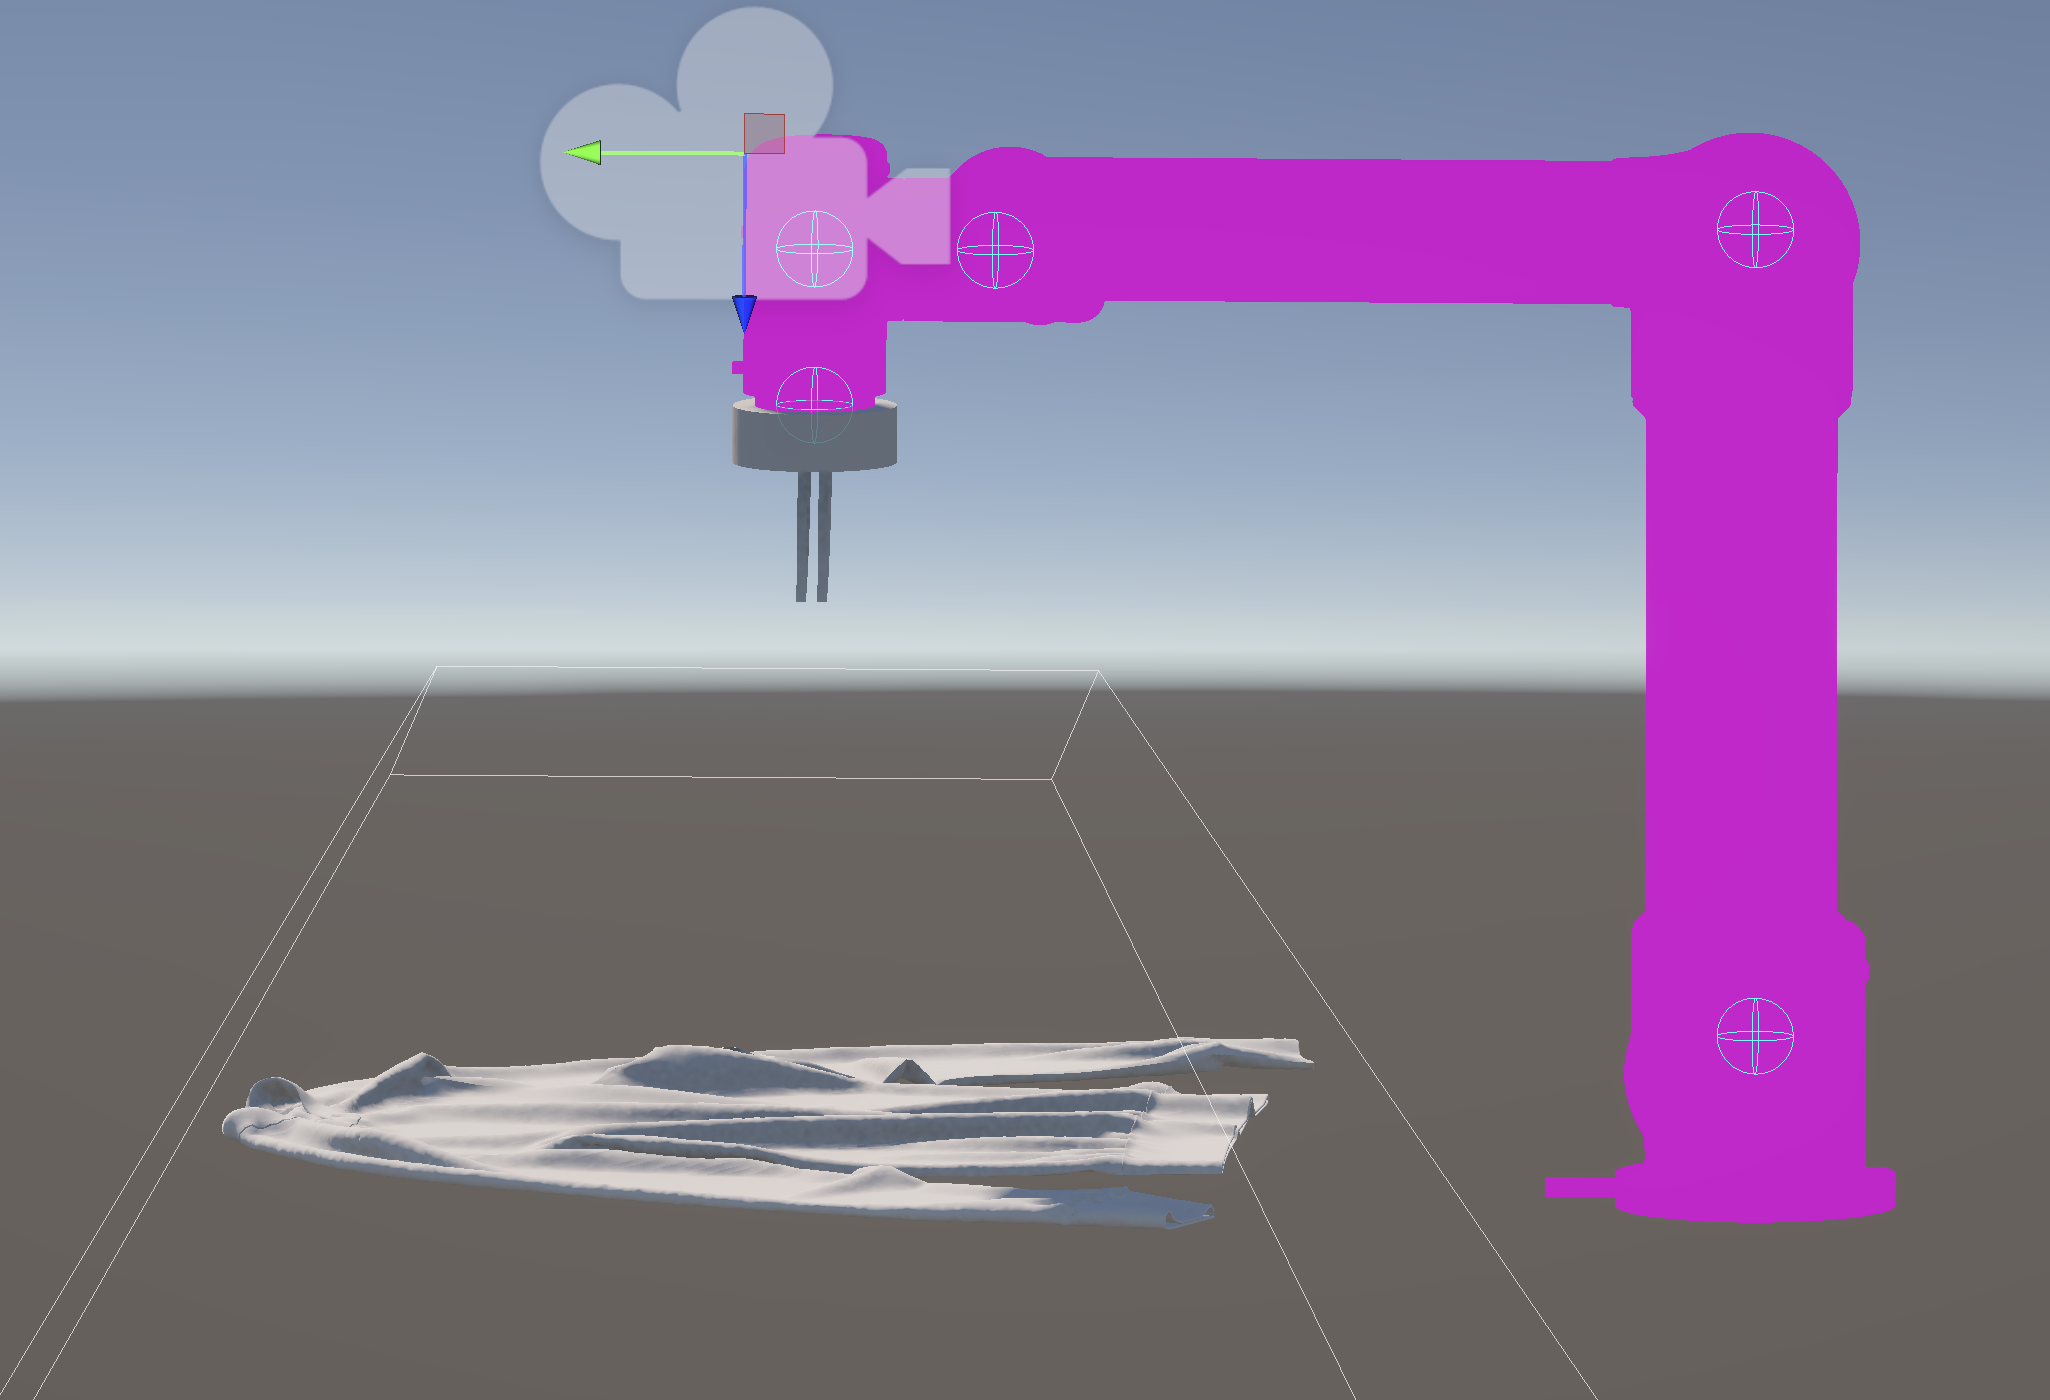
\includegraphics[width=0.75\linewidth]{figures/unity/posizione_home.png}
    \caption{Home Position}
    \label{fig:home position}
\end{figure}

Raggiunta la posizione iniziale, viene acquisita un'immagine RGB del maglione mediante la telecamera simulata. L'immagine viene salvata all'interno della cartella \texttt{Assets} del progetto Unity e successivamente utilizzata come input per la rete neurale sviluppata per l'identificazione dei punti di interesse del capo. In particolare, il modello esegue un'inferenza sull'immagine acquisita ed estrae le coordinate dei punti appartenenti al colletto, ai due polsini e al fondo del maglione, che rappresentano i riferimenti necessari per la generazione della traiettoria di manipolazione.
\begin{figure}[H]
    \centering
    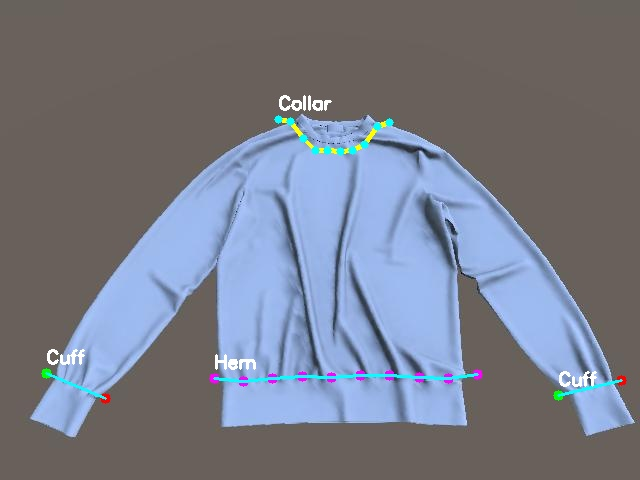
\includegraphics[width=0.75\linewidth]{figures/unity/yolo_inference_unity_result.jpg}
    \caption{Estrazione coordinate tramite rete neurale}
    \label{fig:estrazione coordinate tramite rete neurale}
\end{figure}

Le coordinate prodotte dalla rete neurale vengono quindi elaborate dal nodo \textit{spline\_finale.py}, che costituisce il modulo principale di pianificazione del moto.
I punti vengono presi dallo script python relativi all'inferenza e successivamente inseriti manualmente all'interno nodo precedentemente menzionato.
In una prima fase, i punti vengono convertiti dal sistema di riferimento della telecamera a quello della base del robot mediante opportune trasformazioni geometriche che prevedono l'utilizzo della matrice di trasformazione ricavata da Unity.
Successivamente, il nodo genera una curva spline che interpola i punti estratti, ottenendo una traiettoria continua e sufficientemente regolare da poter essere seguita dal manipolatore.

Per garantire un movimento fluido e privo di brusche variazioni di velocità, la traiettoria geometrica viene parametrizzata temporalmente ed è composta da una serie di profili di velocità trapezoidali che definiscono l'evoluzione temporale del moto dell'end-effector.
A ogni istante di campionamento vengono determinati il riferimento cartesiano desiderato per l'end-effector e la sua posizione attuale, ricavata dallo stato del manipolatore.
Lo stato articolare corrente del manipolatore viene utilizzato per calcolare la posa effettiva dell'end-effector mediante cinematica diretta. Confrontando quest'ultima con la posa desiderata, vengono determinati l'errore di posizione e quello di orientamento.
Il controllo in retroazione integra tali errori nella velocità cartesiana di riferimento, sommando al contributo di velocità pianificata un termine correttivo proporzionale all'errore.
Il Jacobiano del manipolatore viene quindi invertito mediante il metodo Damped Least Squares (DLS), così da poter essere utilizzato per l'ultimo passo della cinematica inversa e ottenere i riferimenti articolari da inviare al robot attraverso i topic ROS~2.

\begin{figure}[H]
    \centering
    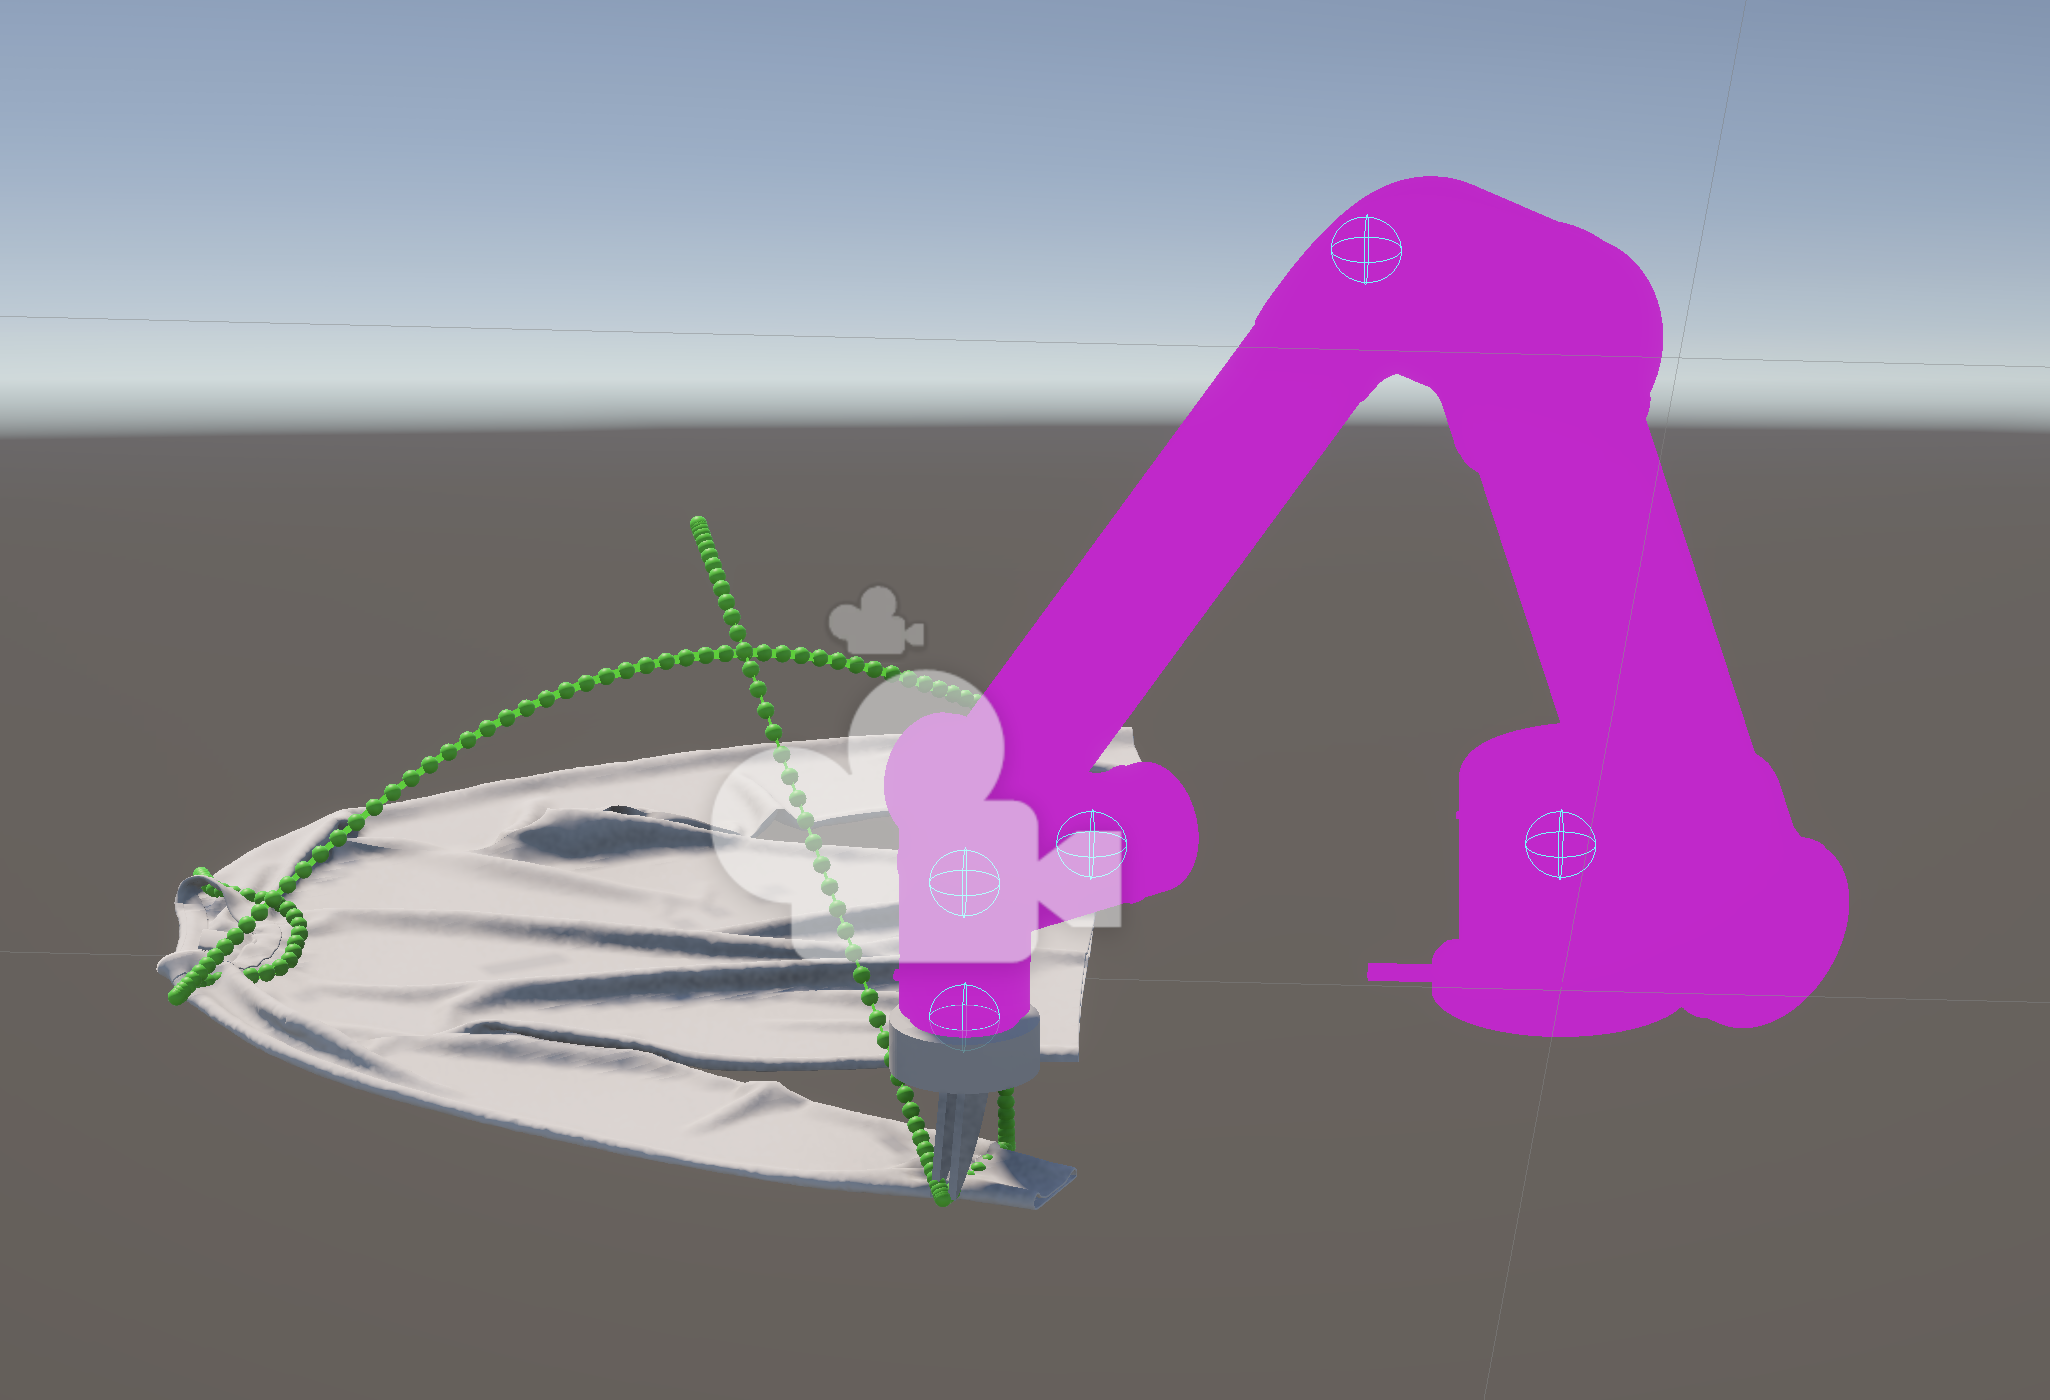
\includegraphics[width=0.75\linewidth]{figures/unity/polsino_sx.png}
    \caption{Visualizzazione traiettoria}
    \label{fig:polsino sx}
\end{figure}

La procedura viene ripetuta a ogni ciclo, aggiornando il comando sulla base dello stato corrente del robot. In questo modo, la pianificazione della traiettoria viene combinata con un controllo in retroazione che mira a ridurre gli errori di inseguimento e a migliorare la precisione del movimento.
Parallelamente all'esecuzione del moto, il nodo pubblica anche l'intera traiettoria pianificata su un topic dedicato. In Unity tale traiettoria viene rappresentata graficamente mediante una sequenza di sfere distribuite lungo il percorso, consentendo una verifica immediata della correttezza della pianificazione e del movimento dell'end-effector rispetto al maglione.

\begin{figure}[H]
    \centering
    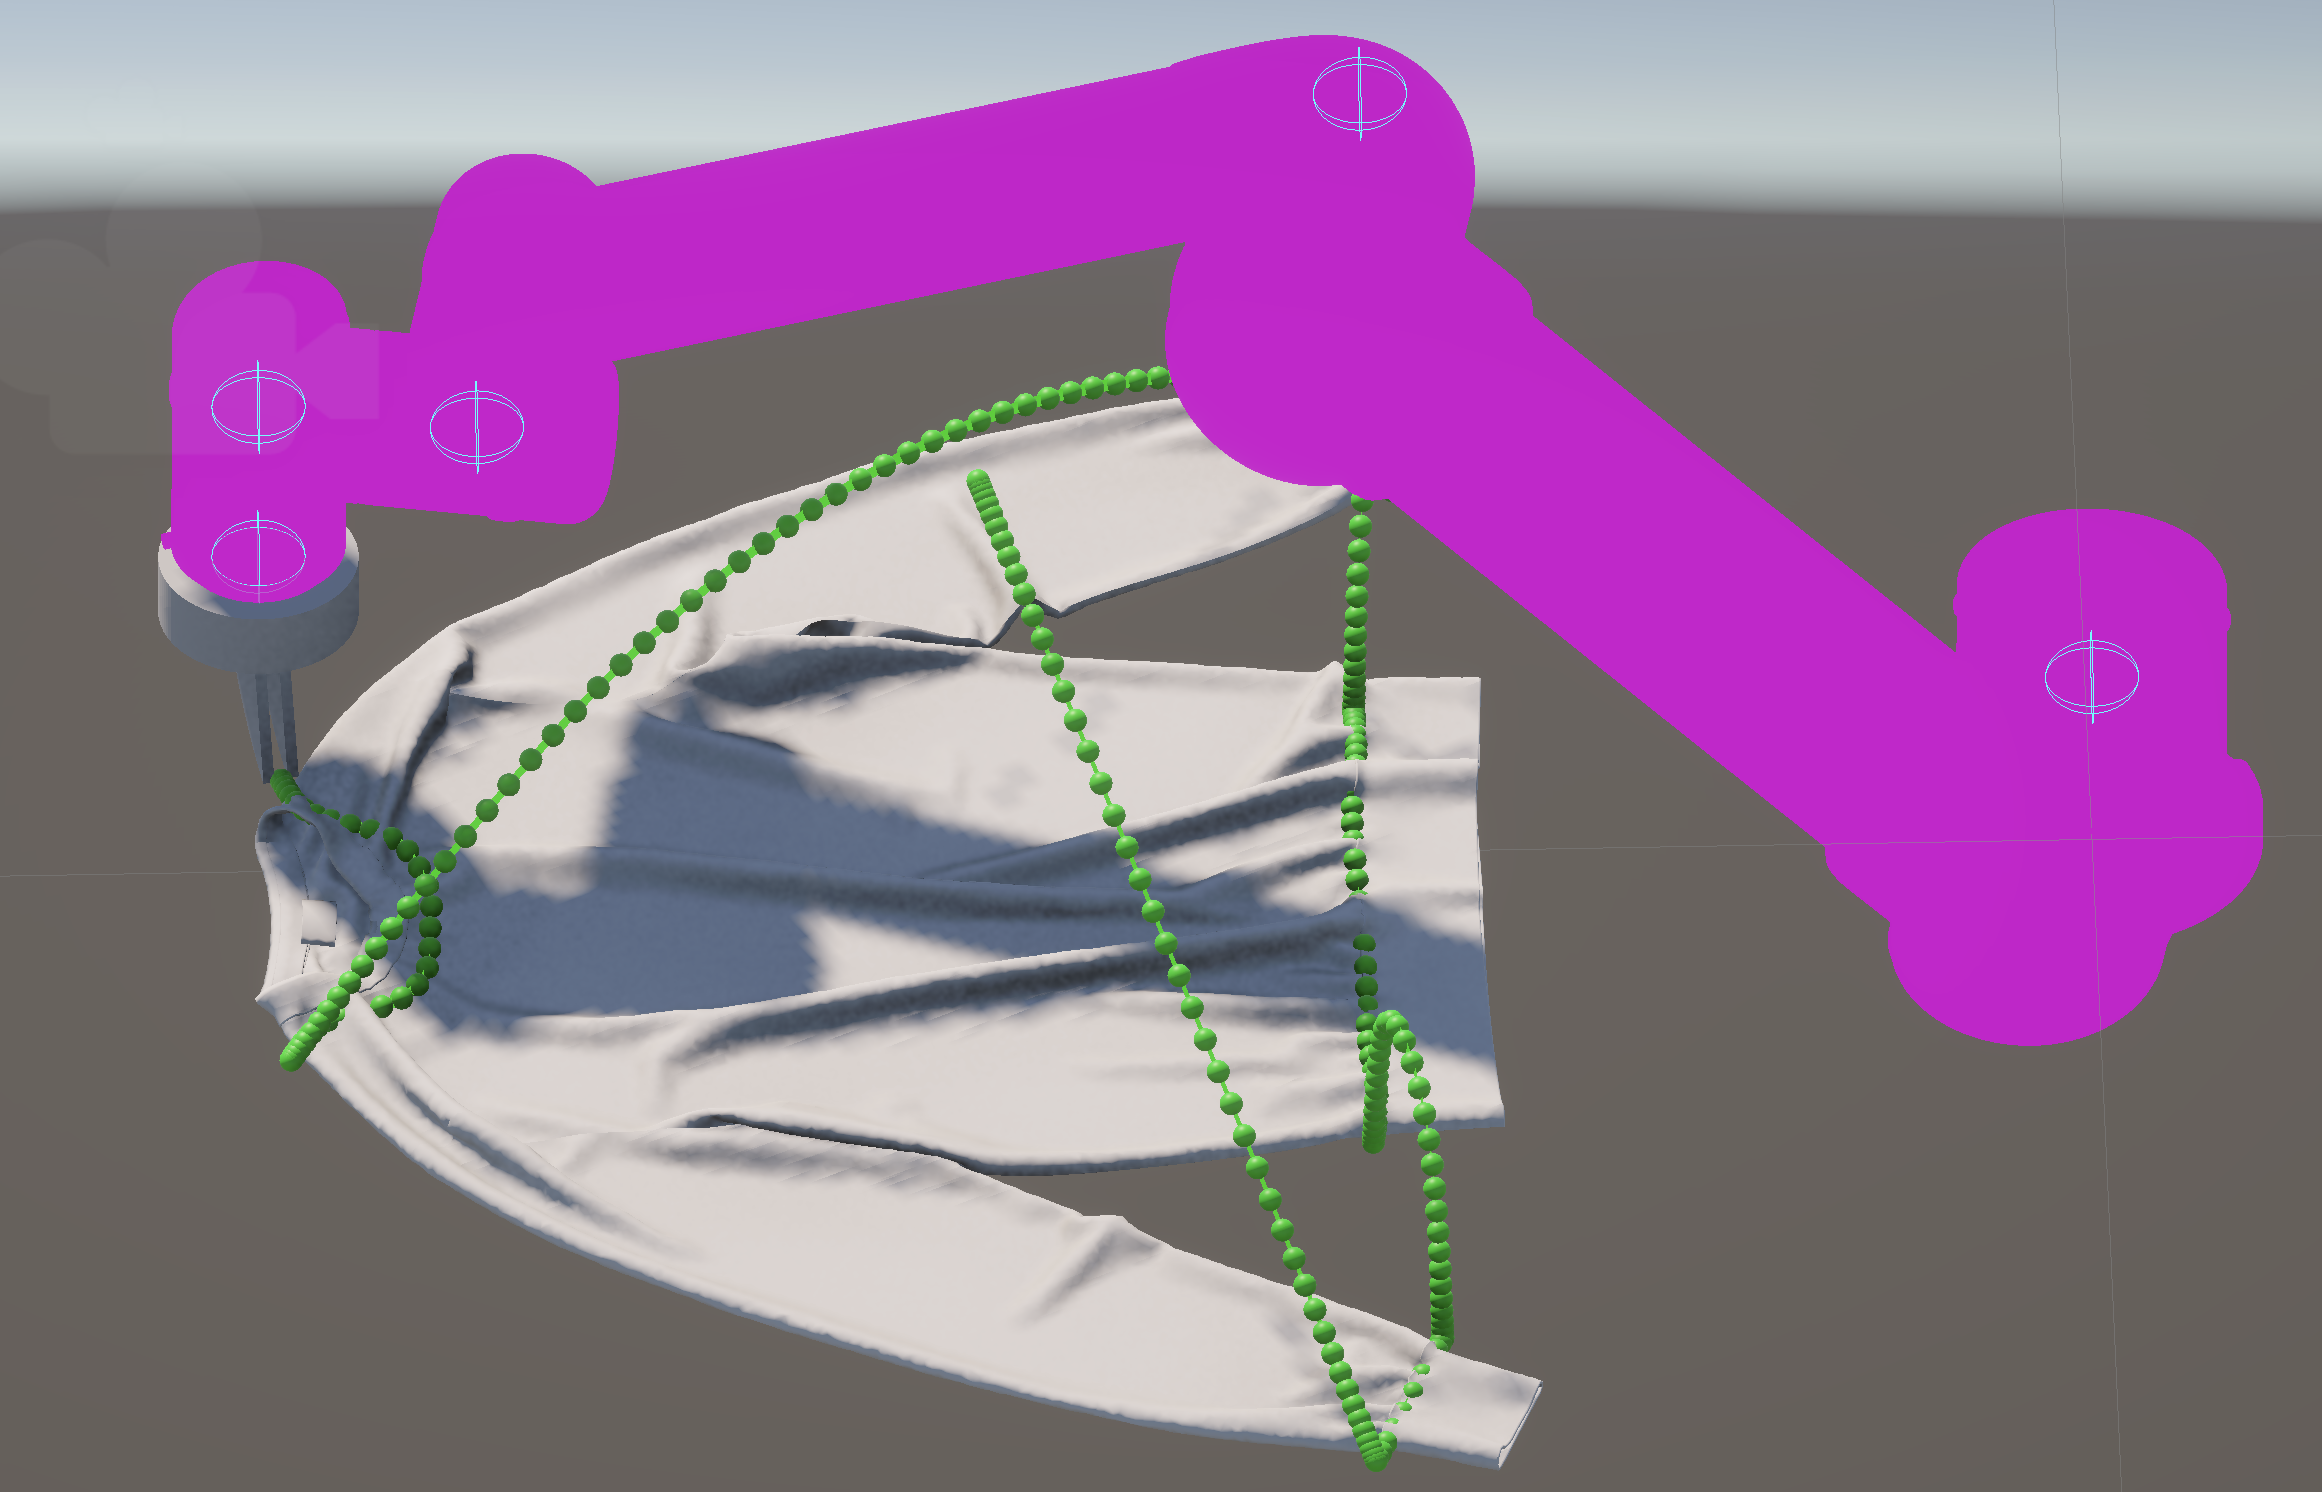
\includegraphics[width=0.75\linewidth]{figures/unity/fine_traiettoria.png}
    \caption{Fine traiettoria}
    \label{fig:fine traiettoria}
\end{figure}